\documentclass[aspectratio=169]{beamer}
\usepackage[utf8]{inputenc}
\usepackage{xcolor,colortbl}
\usepackage{graphics}

\usepackage{tikz}
\usetikzlibrary{positioning,arrows.meta}

\usecolortheme{wolverine}
\definecolor{monerorange}{RGB}{255, 102, 0}
\definecolor{otherorange}{RGB}{253, 188, 148}
\definecolor{redd}{RGB}{253, 150, 179}
\definecolor{grenn}{RGB}{150, 253, 189}
\definecolor{yello}{RGB}{248, 253, 150}
\setbeamercolor*{palette primary}{bg=otherorange}
\setbeamercolor*{frametitle}{bg=otherorange}
\setbeamercolor*{itemize item}{fg=monerorange}
\setbeamercolor*{itemize subitem}{fg=monerorange}
\setbeamertemplate{footline}[frame number]

\newcommand{\com}{\operatorname{Com}}

\title{Triptych}
\subtitle{Logarithmic-sized linkable ring signatures with applications}
\author{Sarang Noether, Ph.D.}
\institute{Monero Research Lab}
\date{17 September 2020}
\begin{document}


\frame{\titlepage}


\begin{frame}{Goal}
We want to build a \textbf{confidential transaction} construction with the following properties:
\begin{itemize}
\item Trust-free setup and parameters
\item Sublinear size scaling with anonymity set
\item Batchable $O(n/\log(n))$ verification
\item Safely compatible with one-time addressing
\item Supports multisignature operations
\end{itemize}
~\\
Our construction is \textbf{Triptych}.
\\~\\
This is joint work with \textbf{Brandon Goodell}.
\end{frame}


\begin{frame}{Our strategy}
\begin{center}
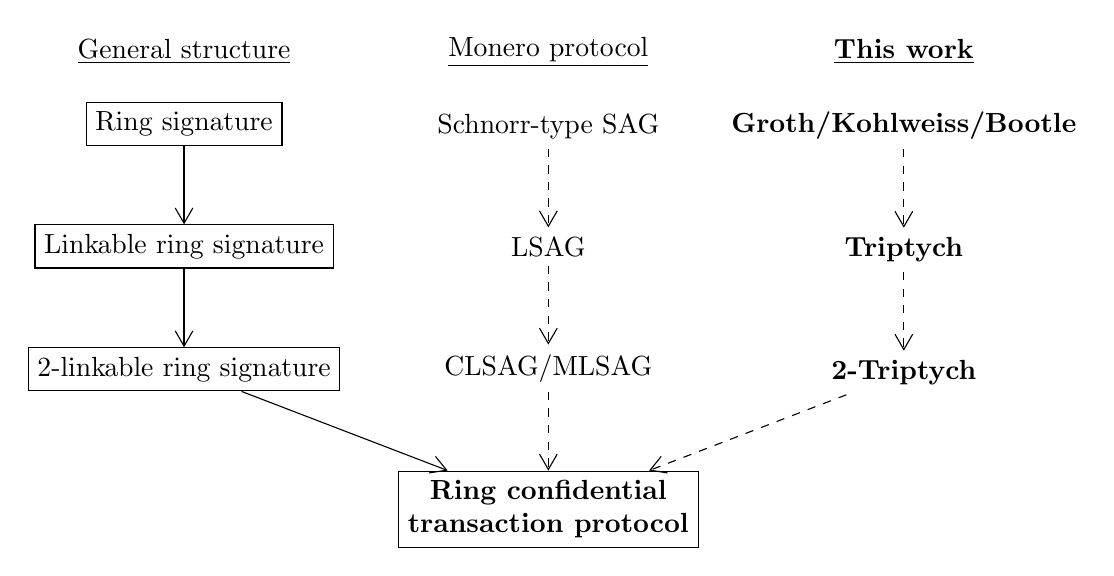
\begin{tikzpicture}[> = {Straight Barb[angle=60:4pt 6]}]
\node (general) {\underline{General structure}};
\node (rs) [draw, below=10pt of general] {Ring signature};
\node (lrs) [draw, below=of rs] {Linkable ring signature};
\node (2lrs) [draw, below=of lrs] {2-linkable ring signature};

\node (monero) [right=50pt of general] {\underline{Monero protocol}};
\node (schnorr) [below=10pt of monero] {Schnorr-type SAG};
\node (lsag) [below=of schnorr] {LSAG};
\node (clsag) [below=of lsag] {CLSAG/MLSAG};
\node (ringct) [draw, below=of clsag, align=center] {\textbf{Ring confidential} \\ \textbf{transaction protocol}};

\node (this) [right=60pt of monero] {\underline{\textbf{This work}}};
\node (gkb) [below=10pt of this] {\textbf{Groth/Kohlweiss/Bootle}};
\node (triptych) [below=of gkb] {\textbf{Triptych}};
\node (2triptych) [below=of triptych] {\textbf{2-Triptych}};

\draw[->] (rs) to (lrs);
\draw[->] (lrs) to (2lrs);
\draw[->] (2lrs) to (ringct);

\draw[->,dashed] (schnorr) to (lsag);
\draw[->,dashed] (lsag) to (clsag);
\draw[->,dashed] (clsag) to (ringct);

\draw[->,dashed] (gkb) to (triptych);
\draw[->,dashed] (triptych) to (2triptych);
\draw[->,dashed] (2triptych) to (ringct);
\end{tikzpicture}
\end{center}
\end{frame}


\begin{frame}{Ring signatures}
A \textbf{ring signature} is a signature construction that signs a message on behalf of a \underline{non-interactive} anonymity set of public keys. The signer knows the secret key to (at least) one of the public keys in the set.
\\~\\
The verifier learns only that one key in the public key set is the signer, but not which one. So
$$\operatorname{Sign}(m,\{M_0,M_1,\ldots\};(l,r)) \to \sigma$$
signs message $m$ such that $M_l$ has $r$ as its secret key, and
$$\operatorname{Verify}(m,\{M_0,M_1,\ldots\},\sigma) \to \{0,1\}$$
verifies.
\end{frame}


\begin{frame}{Ring signatures}
\begin{center}
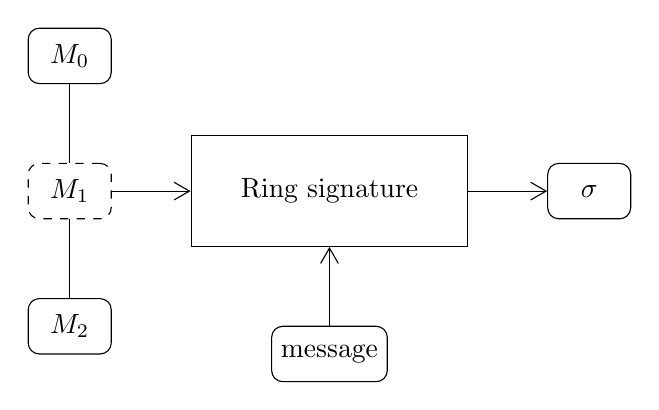
\begin{tikzpicture}[
    box/.style = {draw, minimum width=30pt, minimum height=20pt, rounded corners, align=center},
    dot/.style = {draw, minimum width=30pt, minimum height=20pt, dashed, rounded corners, align=center},
    > = {Straight Barb[angle=60:4pt 6]}
]
\node (rs) [draw, minimum width=100pt, minimum height=40pt] {Ring signature};
\node (M1) [dot, left=of rs] {$M_1$};
\node (M0) [box, above=of M1] {$M_0$};
\node (M2) [box, below=of M1] {$M_2$};
\node (msg) [box, below=of rs] {message};
\node (sig) [box, right=of rs] {$\sigma$};

\draw[-] (M0) to (M1);
\draw[-] (M1) to (M2);
\draw[->] (M1) to (rs);
\draw[->] (msg) to (rs);
\draw[->] (rs) to (sig);
\end{tikzpicture}
\end{center}
\end{frame}


\begin{frame}{Groth/Kohlweiss/Bootle (GKB) ring signatures}
A paper (IACR 2014/764) by \textbf{Groth} and \textbf{Kohlweiss} uses a novel zero-knowledge proving system to build a ring signature construction; it was made more efficient (IACR 2015/643) by \textbf{Bootle} and collaborators.
\\~\\
It builds a sigma protocol for the relation
$$\Big\{\{M_0,\ldots,M_{N-1}\};(l,r) : 0 \leq l < N, M_l = \com(0,r)\Big\}$$
for commitment scheme $\com$, logarithmic in size with $N$.
\\~\\
To transform into a ring signature scheme, use the Fiat-Shamir heuristic and embed the message into the transcript hash.
\end{frame}


\begin{frame}{Properties}
Informally, we want several useful properties. These follow nicely from properties of the underlying sigma protocol.
\\~\\
\begin{itemize}
\item \textbf{Correctness}. Honest signatures always verify.
\begin{itemize}
\item Completeness
\end{itemize}
\item \textbf{Anonymity}. It is not feasible to determine the signing index.
\begin{itemize}
\item Zero knowledge
\end{itemize}
\item \textbf{Unforgeability}. It is not feasible to generate a signature without secret key knowledge.
\begin{itemize}
\item (Special) soundness
\end{itemize}
\end{itemize}
\end{frame}


\begin{frame}{Linkable ring signatures}
What if we wish to identify duplicate signing in a safe way?
\\~\\
A \textbf{linkable ring signature} is a ring signature that adds \underline{linkability} to the signature. Any two valid signatures that link were generated using the same (unknown) secret key. So
$$\operatorname{Link}(\sigma,\sigma') \to \{0,1\}$$
identifies whether two signatures were signed by the same key.
\\~\\
The selection of the anonymity sets can be extremely important for practical security.
\\~\\
It is possible to build constructions that are either dependent or independent of the anonymity set.
\end{frame}


\begin{frame}{Triptych linkable ring signature}
We introduce (IACR 2020/018) \textbf{Triptych} by adding linkability to the GKB construction.
\\~\\
It builds a sigma protocol for the relation
$$\Big\{\{M_0,\ldots,M_{N-1}\}, J;(l,r) : 0 \leq l < N, M_l = \com(0,r), rJ = U\Big\}$$
for globally fixed $U$, where $J$ is the \underline{linking tag}. To check linkability, compare tags.
\\~\\
To transform into a linkable ring signature scheme, use the Fiat-Shamir heuristic and embed the message into the transcript hash.
\end{frame}


\begin{frame}{From GKB to Triptych}
How does the extension from GKB to Triptych work? Treat commitments to zero as public keys, with group generator $G$.
\\~\\
In GKB, we prove knowledge of $r$ such that some commitment is of the form $rG = M$.
\\~\\
In Triptych, we reuse some of this hidden proof data about $r$ to show that $U$ is of the form $rJ = U$. Since $U$ is globally fixed, the prover can only do this if it specifies $J \equiv (1/r)U$, which is a verifiable random function.
\\~\\
Because the sigma protocol is (special) sound and the map $r \mapsto J$ is a bijection, we obtain linkability.
\end{frame}


\begin{frame}{2-linkable ring signatures}
We now extend linkable ring signatures to show knowledge of keys in \underline{parallel lists} of public keys.
\\~\\
The signer provides two lists of public keys, and shows they know the secret key to \underline{both} public keys at the \underline{same} unknown index in both lists.
\\~\\
We will still retain linkability, but only for one of the lists (more on this soon)!
\end{frame}


\begin{frame}{2-linkable ring signatures}
\begin{center}
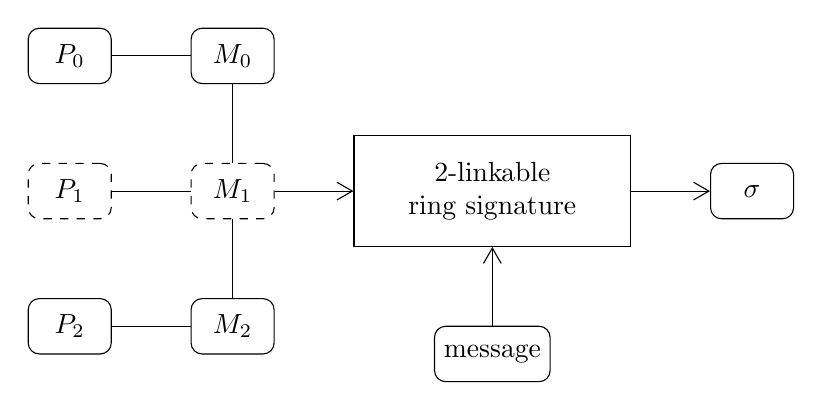
\begin{tikzpicture}[
    box/.style = {draw, minimum width=30pt, minimum height=20pt, rounded corners, align=center},
    dot/.style = {draw, minimum width=30pt, minimum height=20pt, dashed, rounded corners, align=center},
    > = {Straight Barb[angle=60:4pt 6]}
]
\node (rs) [draw, minimum width=100pt, minimum height=40pt, align=center] {2-linkable \\ ring signature};
\node (M1) [dot, left=of rs] {$M_1$};
\node (M0) [box, above=of M1] {$M_0$};
\node (M2) [box, below=of M1] {$M_2$};

\node (P1) [dot, left=of M1] {$P_1$};
\node (P0) [box, above=of P1] {$P_0$};
\node (P2) [box, below=of P1] {$P_2$};

\node (msg) [box, below=of rs] {message};
\node (sig) [box, right=of rs] {$\sigma$};

\draw[-] (M0) to (M1);
\draw[-] (M1) to (M2);
\draw[-] (M0) to (P0);
\draw[-] (M1) to (P1);
\draw[-] (M2) to (P2);
\draw[->] (M1) to (rs);
\draw[->] (msg) to (rs);
\draw[->] (rs) to (sig);
\end{tikzpicture}
\end{center}
\end{frame}


\begin{frame}{Triptych 2-linkable ring signature}
We modify Triptych to construct a 2-linkable ring signature; this can even be done more generally.
\\~\\
It builds a sigma protocol for the relation
\begin{multline*}
\Big\{\{M_0,\ldots,M_{N-1}\}, \{P_0,\ldots,P_{N-1}\}, J;(l,r,s) : \\
0 \leq l < N, M_l = \com(0,r), P_l = \com(0,s), rJ = U\Big\}
\end{multline*}
that now includes two public key lists.
\\~\\
While we need new proof data about the secret key $s$, we can reuse existing proof data about the index $l$.
\end{frame}


\begin{frame}{Ring confidential transaction protocol}
We wish to build a \textbf{confidential transaction} protocol that:
\begin{itemize}
\item Consumes multiple transaction outputs
\item Generates multiple transaction outputs
\item Hides output amounts
\item Hides signing indices
\item Supports in-band stealth addressing
\end{itemize}
~\\
We can do this using arbitrary 2-linkable ring signatures, like 2-Triptych or CLSAG.
\end{frame}


\begin{frame}{Ring confidential transaction protocol}
Define a Pedersen commitment $\com(v,r) \equiv vH + rG$ for group generators $G,H$.
\\~\\
We wish to generate a transaction consuming $W$ existing outputs and generating $T$ new outputs.
\\~\\
Form a single anonymity set of $N \geq W$ public keys $\{M_k\}_{k=0}^{N-1}$ such that for a secret index set $\{l_u\}_{u=0}^{W-1} \subset [0,N)$, we have $M_{l_u} = r_uG$ for all $0 \leq u < W$, where each $r_u$ is a secret key.
\end{frame}


\begin{frame}{Ring confidential transaction protocol}
Let's see an example, where $W = 3$ and $N \geq 3$ is arbitrary.

\begin{center}
\begin{tikzpicture}
\node (M0) {$M_0$};
\node (M1) [right=of M0] {$M_1$};
\node (M2) [right=of M1] {$M_2$};
\node (dots) [right=of M2] {$\cdots$};
\node (MN1) [right=of dots] {$M_{N-1}$};
\node (r0) [below=of M2] {$r_0$};
\node (r1) [below=of M0] {$r_1$};
\node (r2) [below=of MN1] {$r_2$};

\draw[-, dashed] (r0) to (M2);
\draw[-, dashed] (r1) to (M0);
\draw[-, dashed] (r2) to (MN1);
\end{tikzpicture}
\end{center}

So the secret index set is $\{l_u\}_{u=1}^{W-1} = \{2, 0, N-1\}$.
\end{frame}


\begin{frame}{Ring confidential transaction protocol}
Each of the $0 \leq u < W$ consumed outputs comes associated with a commitment to an amount $a_u$:
$$P_{l_u} \equiv \com(a_u,s_u)$$

Because the Triptych proving system assumes knowledge of commitments to zero, form an \underline{commitment offset} for each consumed output, with the same value but a uniformly random mask:
$$P'_u \equiv \com(a_u,s'_u)$$

This gives these commitments to zero:
$$P_{l_u} - P'_u = \com(a_u,s_u) - \com(a_u,s'_u) = \com(0,s_u-s'_u)$$
\end{frame}


\begin{frame}{Ring confidential transaction protocol}
Generate $0 \leq j < T$ new outputs, where each has an associated amount commitment (and range proof):
$$Q_j \equiv \com(b_j,t_j)$$
We choose, for $1 \leq j < T$, random masks $t_j$. Then we set
$$t_0 \equiv \sum_{u=0}^{W-1} s'_u - \sum_{j=1}^{T-1} t_j$$
such that, if the consumed and generated amounts balance, the verifier can perform this check:
$$\sum_{u=0}^{W-1} P'_u - \sum_{j=0}^{T-1} Q_j = 0$$
\end{frame}


\begin{frame}{Ring confidential transaction protocol}
Finally, generate a signature for each of the $0 \leq u < W$ consumed outputs, using the following 2-Triptych relation inputs:
$$\Big\{\{M_k\}_{k=0}^{N-1},\{P_k-P'_u\}_{k=0}^{N-1},(1/r_u)U; (l_u,r_u,s_u-s'_u)\Big\}$$
To verify such a transaction:
\begin{itemize}
\item Verify each of the linkable ring signatures
\item Perform a linking test among all signatures
\item Ensure the balance check succeeds
\item Verify all output range proofs
\end{itemize}
\end{frame}


\begin{frame}
\centering
\includegraphics[width=\textwidth]{protocol.jpeg}
\end{frame}


\begin{frame}{Comparison}
\begin{center}
\renewcommand{\arraystretch}{1.5}
\begin{tabular}{|r|ccccc|}
\hline
& Size & Verification & Batching & Addressing & Aggregation \\
\hline
\textbf{Triptych} & \cellcolor{grenn} $O(\log N)$ & \cellcolor{yello} $O(N/\log N)$ & \cellcolor{grenn} yes & \cellcolor{grenn} yes & \cellcolor{redd} no \\
Arcturus & \cellcolor{grenn} $O(\log N)$ & \cellcolor{yello} $O(N/\log N)$ & \cellcolor{grenn} yes & \cellcolor{grenn} yes & \cellcolor{grenn} yes \\
CLSAG & \cellcolor{redd} $O(N)$ & \cellcolor{redd} $O(N)$ & \cellcolor{redd} no & \cellcolor{grenn} yes & \cellcolor{redd} no \\
Lelantus & \cellcolor{grenn} $O(\log N)$ & \cellcolor{yello} $O(N/\log N)$ & \cellcolor{grenn} yes & \cellcolor{redd} no & \cellcolor{redd} no \\
Omniring & \cellcolor{grenn} $O(\log N)$ & \cellcolor{yello} $O(N/\log N)$ & \cellcolor{redd} no & \cellcolor{grenn} yes & \cellcolor{grenn} yes \\
RingCT 3.0 & \cellcolor{grenn} $O(\log N)$ & \cellcolor{yello} $O(N/\log N)$ & \cellcolor{grenn} yes & \cellcolor{grenn} yes & \cellcolor{yello} padded \\
\hline
\end{tabular}
\end{center}

\begin{center}
This chart is intentionally oversimplified.
\end{center}
\end{frame}


\begin{frame}{Conclusions}
\textbf{Triptych} is a zero-knowledge proving system that can be used to construct a linkable (and 2-linkable!) ring signature construction, which in turn can power a confidential transaction model. It:
\begin{itemize}
\item Requires no trusted setup or parameters
\item Scales logarithmically in size (with superior size for reasonable anonymity sets)
\item Scales (sub)-linearly in verification time, with batching
\item Is fully compatible with in-band stealth addressing
\item Supports multisignature operations via Paillier secret sharing
\end{itemize}
\begin{center}
~\\
\textbf{\Large Questions?}
\end{center}
\end{frame}


\end{document}